\documentclass[tikz,border=2]{standalone}
\usetikzlibrary{shadows,arrows,shapes,positioning,calc,backgrounds,fit,automata}
%
%%%%%%%%%%%%%%%%%%%%%%%%%%%%%%%%%%%%
%% Common preamble
%%%%%%%%%%%%%%%%%%%%%%%%%%%%%%%%%%%%
% PAGE
%% \usepackage{fullpage}
% FONTS
\usepackage{lmodern} % enhanced version of computer modern
\usepackage[T1]{fontenc} % for hyphenated characters
%% \usepackage{gillius2}
%% \renewcommand{\familydefault}{\sfdefault}
\usepackage{amssymb} % for \checkmark
\usepackage{mathtools} % contains amsmath which comes with align
\usepackage{amsthm}
%%\usepackage{enumitem}
\usepackage{microtype} % some compression
%%%%%%%%%%%%%%%%%%%%%%%%%%%%%%%%%%%%
\usepackage{subfig}
\usepackage{tikz}
\usetikzlibrary{spy,shadows,arrows,shapes,positioning,calc,backgrounds,fit,automata}
\newcommand{\score}{\text{score}}

\definecolor{myblue}{HTML}{C5E0DC}
\definecolor{vtblue}{HTML}{557082}
\definecolor{hokie}{HTML}{660000}
\definecolor{hokieRed}{HTML}{980000}

\definecolor{col1}{HTML}{D53E4F}
\definecolor{col2}{HTML}{F46D43}
\definecolor{col3}{HTML}{FDAE61}
\definecolor{col4}{HTML}{FEE08B}
\definecolor{col5}{HTML}{E6F598}
\definecolor{col6}{HTML}{ABDDA4}
\definecolor{col7}{HTML}{66C2A5}
\definecolor{col8}{HTML}{3288BD}

\newcommand{\dunder}[1]{\underline{\underline{#1}}}
\newcommand{\dmax}{d_{\max}}
\newcommand{\cost}{\text{cost}}
%\newcommand{\comment}[1]{{\color{red}#1}}
\newcommand{\wmin}{w_{\min}}
\newcommand{\copt}{C_{\text{OPT}}}
\newcommand{\TikZ}{Ti\textit{k}Z\xspace}
\newcommand{\tuta}{\emph{T. absoluta}}
\newcommand{\prempt}{\textsc{PREMpT}}
\newcommand{\parnode}[1]{\parbox{3cm}{\centering #1}}

%%
%% This ``scales'' the font. Don't extend too much beyond 128x96
%% Uncomment the next line for default sizes:
%% \setbeamercolor{block title}{use=structure,fg=white,bg=black!75!white}
%% \setbeamercolor{block body}{use=structure,fg=black,bg=black!10!white}
%%
%% ----------------------------------------------------------------------
%%
\begin{document}
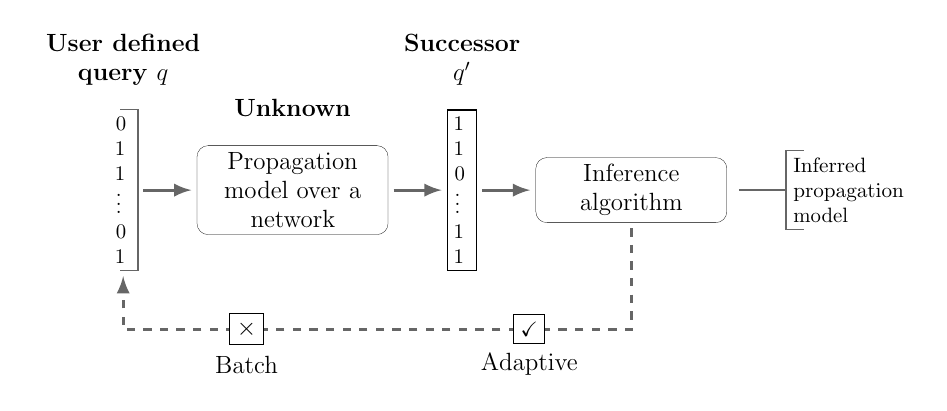
\begin{tikzpicture}
[scale=.75,auto,transform shape,
edge/.style={black!60,>=latex, shorten >=2pt, shorten <=2pt, line width=.4mm},
block/.style={draw=black,ultra thin,rounded corners}]
%%
\node[] (q) {\parbox{.25cm}{0\\1\\1\\$\vdots$\\0\\1}};
%%
\node [above of=q,shift={(0,1.2)},font=\large] {\parnode{\bf User defined
query~$q$}};
\node (gds) [block,right=of q,font=\large] {\parnode{Propagation model over a
network}};
\node [above of=gds,shift={(0,.4)},font=\large] {\parnode{\bf Unknown}};
\draw[edge,->] (q.east) -- (gds);
\draw [black!60,line width=.2mm] (q.east) |- (q.north east) -- +(-.3,0);
\draw [black!60,line width=.2mm] (q.east) |- (q.south east) -- +(-.3,0);
\node[right=of gds,draw] (qp) {\parbox{.25cm}{1\\1\\0\\$\vdots$\\1\\1}};
%%
\node [above of=qp,shift={(0,1.2)},font=\large] {\parbox{2cm}{\centering\bf Successor 
$q'$}};
\node (inf) [block,right=of qp,font=\large] {\parnode{Inference algorithm}};
\node (result) [right=of inf] {\parbox{2cm}{Inferred propagation model}};
%%
\draw[edge,->] (gds.east) -- (qp);
\draw[edge,->] (qp) -- (inf);
\draw [edge,line width=.2mm] ($(inf.east)+(.2,0)$) -- (result) -|
(result.north west) -- +(.4,0);
\draw [edge,line width=.2mm] (result) -| (result.south west) -- +(.4,0);
\draw [edge,dashed,->] (inf) |- ($(q.south)+(0,-1)$) -- (q);
\node (yes) at (inf.south) [right,black,shift={(-2,-1.8)},fill=white,draw] {$\checkmark$};
\node (no) at (q.south|-yes) [right,black,shift={(1.8,0)},fill=white,draw]
{\large$\times$};
\node [font=\large,below of=yes,shift={(0,.4)}] {Adaptive};
\node [font=\large,below of=no,shift={(0,.4)}] {Batch};
\end{tikzpicture}
\end{document}
